\documentclass[letterpaper,10pt]{article}

\usepackage{titling}
\usepackage{listings}
\usepackage{url}
\usepackage{setspace}
\usepackage{subfig}
\usepackage{sectsty}
\usepackage{pdfpages}
\usepackage{colortbl}
\usepackage{multirow}
\usepackage{multicol}
\usepackage{relsize}
\usepackage{amsmath}
\usepackage{fancyvrb}
\usepackage{amsmath,amssymb,amsthm,graphicx,xspace}
\usepackage[titlenotnumbered,noend,noline]{algorithm2e}
\usepackage[compact]{titlesec}
\usepackage{XCharter}
\usepackage[T1]{fontenc}
\usepackage{tikz}
\usetikzlibrary{arrows,automata,shapes,trees,matrix,chains,scopes,positioning,calc}
\tikzstyle{block} = [rectangle, draw, fill=blue!20, 
    text width=2.5em, text centered, rounded corners, minimum height=2em]
\tikzstyle{bw} = [rectangle, draw, fill=blue!20, 
    text width=4em, text centered, rounded corners, minimum height=2em]

\newcommand{\CPP}{C\nolinebreak\hspace{-.05em}\raisebox{.4ex}{\tiny\bf +}\nolinebreak\hspace{-.10em}\raisebox{.4ex}{\tiny\bf +}}
\def\CPP{{C\nolinebreak[4]\hspace{-.05em}\raisebox{.4ex}{\tiny\bf ++}}}

\let\LaTeXtitle\title
\renewcommand{\title}[1]{\LaTeXtitle{\textsf{#1}}}


\addtolength{\oddsidemargin}{-1.000in}
\addtolength{\evensidemargin}{-0.500in}
\addtolength{\textwidth}{2.0in}
\addtolength{\topmargin}{-1.000in}
\addtolength{\textheight}{1.75in}
\addtolength{\parskip}{\baselineskip}
\setlength{\parindent}{0in}
\renewcommand{\baselinestretch}{1.5}

\singlespace

\begin{document}

\lecture{ 34 --- DevOps: Configuration}{\term}{Patrick Lam \& Jeff Zarnett}

\section*{DevOps for P4P}
So far, we've talked almost exclusively about one-off computations:
you want to figure out the answer to a question, and you write code to
do that and when it's finished, you are done. 
The course assignments have been like that, for instance. There are lots
of programs in the world that are solely executed on-demand. Still, a lot
of the time we want to keep systems running over time. That is, a service
that is available (if not always then close to it) and responds to requests
whenever they may happen to arrive. That gets us
into the notion of operations. Your service or product is more likely than 
ever to have at least some component that's server side (whether hosted
in a cloud service or not) that's under your control. And that server side
component is something you want to keep running as it's supposed to be 
``generally available''.

The theme in this topic will be using software development skills in
operations (e.g., system administration, database management, etc). This
does have some relevance, because the operations (or IT, if you prefer)
processes and procedures, while different from development, have some
similarities. 

Even when we've talked about multi-computer tools like cloud
computing, it still has not been in the context of keeping your
systems operational over longer timescales. The trend today is away
from strict separation between a development team, which writes the
software, and an operations team, which runs the software and infrastructure.

\begin{center}
	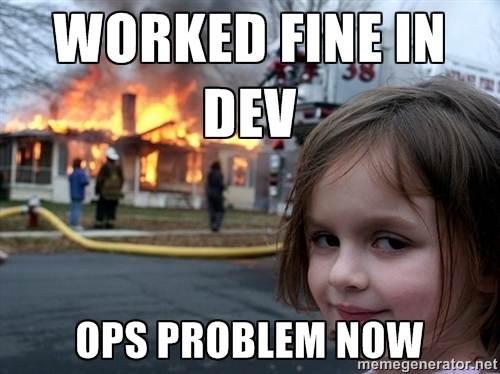
\includegraphics[width=0.45\textwidth]{images/devops.jpg}
\end{center}

The separation is totally nonexistent at the typical startup company. There isn't the money to pay for separate developers and operations teams. And in the beginning there's probably not that many servers, just a few demo systems, test systems, etc... but it spirals out from there. You're not really going to ask the sales team to manage these servers, are you? So, there's DevOps, also sometimes called Software Reliability Engineering.

Is DevOps a good idea? Like most ideas it can be used for both good and evil. There's a lot to be said for letting the developers be involved in all the parts of the software from development to deployment to management to training the customers. Developers can learn a lot by having to do these kinds of things, and be motivated to make proper management and maintenance tools and procedures. If we make the pain of operations felt by developers, they might do something about it. If it's the problem of another team, somehow those tickets just never make it to the top of the backlog.

As the company grows, you might think about whether a dedicated operations team is preferable. That may be sensible, but shifting all workload to the operations team probably isn't ideal for the reasons above. And it is probably not scalable, either. If the operations team has to be involved in everything they can quickly become a bottleneck and everyone is happier if the development teams are able to solve their own problems instead of opening tickets and then hassling people to please just do the thing.

\paragraph{Continuous Integration.} 
This is now a best practice -- each change (or related group of changes) is built and tested to evaluate it. Once upon a time, putting the code changes together didn't happen on every build, but nightly or otherwise. That was a weird time when builds were slow and expensive. I think we're past that now, especially given that we have use of version control, good tests, and scripted deployments.
It works like this:
\begin{itemize}
\item pull code from version control;
\item build;
\item run tests;
\item report results.
\end{itemize}
What's also key is a social convention to not break the build. These things get done automatically on every commit and the results are sent to people by e-mail, Slack, Teams, or whatever you use. 

Thanks to Chris Jones and Niall Murphy for some inputs for following points.

\subsection*{Configuration as Code}
Systems have long come with complicated configuration options. 
Sendmail is particularly notorious, but apache and nginx aren't super
easy to configure either. But the environment that you're running your code in is also a kind of configuration. Furthermore, it's an excellent idea to have tools for configuration. It's not enough to just have a wiki page or github document titled ``How to Install AwesomeApp'' (fill in name of program here). Complicated means mistakes and people will forget steps. Don't let them make mistakes: make it automatic. The first principle is to treat \emph{configuration as code}. 
Therefore:
\begin{itemize}
\item use version control on your configuration.
\item implement code reviews on changes to the configuration.
\item test your configurations: that means that you check that they
  generate expected files, or that they spawn expected
  services. (Behaviours, or outcomes.) Also, configurations should
  ``converge''. Unlike code, they might not terminate; we're talking
  indefinitely-running services, after all. But the CPU usage should
  go down after a while, for instance.
\item aim for a suite of modular services that integrate together smoothly.
\item refactor configuration files (Puppet manifests, Chef recipes, etc);
\item use continuous builds
\end{itemize}

One particular example of applying all those principles to infrastructure
is Terraform. Its whole purpose is to manage your config as codes
situation where you want to run your code using a cloud provider (e.g., AWS), 
then you can control the infrastructure using Terraform: you write the
configuration files that say you want this service with these permissions
(and any other details) and then you can apply that configuration easily. 
Even beyond that, you can ask Terraform to manage things like who has access
to your GitHub repositories and who is in what groups (e.g., reviewers).

Terraform does support a ``plan'' operation so it can tell you what it will
do, so you can verify that, before anything is actually changed. The plan can also tell you expected changes in terms of cost, which both helps verify that we aren't about to give all our money to Jeff Bezos but also that a small change is actually small. If you are happy with the change, apply it! 

The plan operation isn't perfect as things can change between the plan and apply steps, and some things like unique identifiers are really only known if they are created. Non-destructive changes are generally easy to deal with; just make another PR that corrects it. Destructive changes, however...

It's easy for very bad things to happen with Terraform as well: you could accidentally tell it you want to destroy all GitHub groups and it will gladly carry it out. This has the side effect of causing some people to message you on Slack in a panic, thinking that the removal of their GitHub access is actually a sign they are being fired. They were not. But I see why they were worried, honestly. Restoring some information in destructive changes might not be as easy as just reverting the change: if you told your tool to destroy a database, reverting the change will re-create the database, but not its contents. You took backups, right?

\subsection*{Common Infrastructure}
Using tools to manage the infrastructure is a good start, but it also matters how services use it. You should view different parts of your infrastructure as having an interface and communication is done exclusively via the interface or API. This reduces the coupling between different components, and, as we've discussed, allows you to scale the parts that need scaling. 

Try to avoid not-invented-here syndrome: it is usually better to use an existing tool -- whether open-source, commercial, or provided by your cloud platform -- than to roll your own. Some examples might be:
\begin{itemize}
\item Storage: some sort of access layer (e.g., MongoDB or S3);
\item Naming and discovery (e.g., Consul)
\item Monitoring (e.g., Prometheus)
\end{itemize}

However, be prepared to build your own tools if needed. Sometimes what you want, or need, doesn't exist (yet). Think carefully about whether this service that is needed is really part of your core competence and whether creating it adds sufficient value to the business. It's fun to make your own system and all, but are you doing what you're best at? 

Think extra carefully if you plan to do roll your own anything that is security or encryption related. I'm just going to say that unless you have experts on staff who know the subject really well and you're willing to pay for external audits and the like, you're more likely to end up with a terrible security breach than a terrific secure system. 

As a second followup soapbox point to that: if what you are looking for doesn't exist, there might be a reason, Maybe the reason is that you are the first to think of it, but consider the possibility that it's not that good of an idea (either due to inefficiency or just not being great in principle). 

With that said, big platforms like AWS are constantly launching new tools that might do what you want and the best strategy may be just wait until the managed service is provided for you. Patience can be rewarded, in this regard, and you can easily feel very frustrated by investing a lot of effort into planning, building, and launching a feature only to find that your provider has rendered it redundant immediately thereafter.

\subsection*{Naming}
Naming is one of the hard problems in computing. There is a saying that there are only two hard things in computers: cache invalidation, naming things, and off by one errors.  There are a
lot of ways to name things. Naming is necessary for resources of all kinds. There's the Java package approach of infinite dots for your server: live.application.customer.webdomain.com or however you want to call it. Whatever we pick, though, names need to be consistent or at least close to it.

Debates often rage in companies about whether teams, services, or anything else can or should have names that are ``meaningful'' or not. There's arguments for both sides: if the service is called \texttt{billing} it may be helpful in determining what it does, more so than if it were called \texttt{potato}. But there's the possibility of confusion around whether when you say the word billing you mean the service or the team. And what if we want to replace the billing service with a new one? Is it \texttt{billing2}? All of this presupposes, also, that your service does exactly one thing. What if the service is ``billing and accounting''; do you rename it? Is accounting just folded into billing? How do we even decide such things? 

Allegedly-descriptive names aren't always the easiest to figure out either. I've seen examples where the teams are called (anonymized a bit) ``X infrastructure'' and ``X operations'' and I'd estimate that 35\% of queries to each team result in a reply that says that the question should go to the other team. It gets worse when a team is responsible for a common or shared component (e.g., library). 

The \textit{real} solution to this kind of problem at least in my opinion, is similar to the idea of service discovery: we need a tool that provides directory information: if I want to know about \texttt{potato} I need to be able to look it up and have it send me to the right place. Tools for this, like OpsLevel, exist (even if they do much more than this). Such tools can also give some information about service maturity -- are you using deprecated things, do you have unpatched security vulnerabilities, is there enough test coverage...?

There are potential morale implications for insisting on boring names for teams and services. A team that has named itself after some mythological name or fictional organization can have some feeling of identity in it -- Avengers, Assemble -- and that can be valuable. 

\subsection*{Servers as cattle, not pets}
By servers, I mean servers, or virtual machines, or containers. It's much better to have a reproducible process for deployment of a server than doing it manually every single time. The amount of manual intervention should be minimized and ideally zero. If this is done you can save a lot of hours of time, reduce errors, and allow for automatic scaling (starting and stopping servers depending on demand).

The title references the idea that cattle are dealt with as a herd: you try to get the whole group to move along and do what they need. Pets are individuals, though, and you'll treat them all differently. This amount of individual attention quickly becomes unmanageable and there's no reason why you should worry about these differences in a world with virtualization (containers) or similar. 

As with managing infrastructure, I'll give a specific example: Kubernetes. This is used to automate deploying and scaling of applications. This means you don't have to manually manage them; if you want to deploy a new version of a container, just tell Kubernetes to do it. The part about how it does so is that it provides a framework for your environment. It can do load balancing, automatic rollouts and reverts (if something went wrong), will figure out what instances run on what hardware, check the health of instances, replace them if they die, and more.

\paragraph{Canarying.} Rather than just deploying all at once, one thing we could do to test a deployment is referred to as canarying. There are two ways this can happen. One is to deploy new software alongside the existing software and redirect a small fraction of traffic  to the new service and evaluate it. If it's good, keep or increase the fraction of traffic; otherwise, take it out of service. The other way of canarying is upgrading some, but not all, instances of the service and checking if they are working as expected.

This is also called ``test in prod''. Sometimes you just don't know how code is really going to work until you try it. After, of course, you use your best
efforts to make sure the code is good. But real life is rarely like the test system. I've seen many operations that work beautifully in the development environment where there are 100~000 records... and time out in production where there are 10~000~000. But for canarying deployments of the second kind, the basic steps:
\begin{itemize}
\item stage for deployment;
\item remove canary servers from service;
\item upgrade canary servers;
\item run automatic tests on upgraded canaries;
\item reintroduce canary servers into service;
\item see how it goes!
\end{itemize}

Of course, you should implement your system so that rollback is possible. If the canary deployment results in changes to the database table structure and this database is shared amongst all servers, trying to deploy the change can break the old servers and leave a rollback implausible because 



\paragraph{Containers.} What about containers? Well, let's see how we got there first. In the beginning, you had services where you installed the binaries and config files by hand. That sucked. So there were packages; a package includes everything the program needs (including a list of dependencies) and a script to install it and set it up. Great! But if you just install multiple services on the same machine you don't get isolation and you might have incompatible versions of dependencies and you're in RPM hell (see also: JAR hell, classloader hell, and DLL hell).

Right, so instead you say you should have virtual machines: you configure the VM parameters and install the guest OS and set it up (and you can copy-paste the initial image, which helps) but for every application you have a guest operating system running underneath. Maybe we don't need every app to have its own guest OS; why do we have to install the same security patch ten times...?

Containerization gives many of the advantages of this separation, but without nearly so much overhead of the guest operating systems (both its maintenance and runtime costs). Containers are run by a container engine so there is some abstraction of the underlying hardware, and the container is assembled from a specification that says what libraries, tools, etc. are needed. And thus when the container is built and deployed it is sufficiently isolated but shares (in read only mode) where it can. So a container is a very lightweight VM, in some sense. See this diagram from~\cite{netappcontainer}:

\begin{center}
	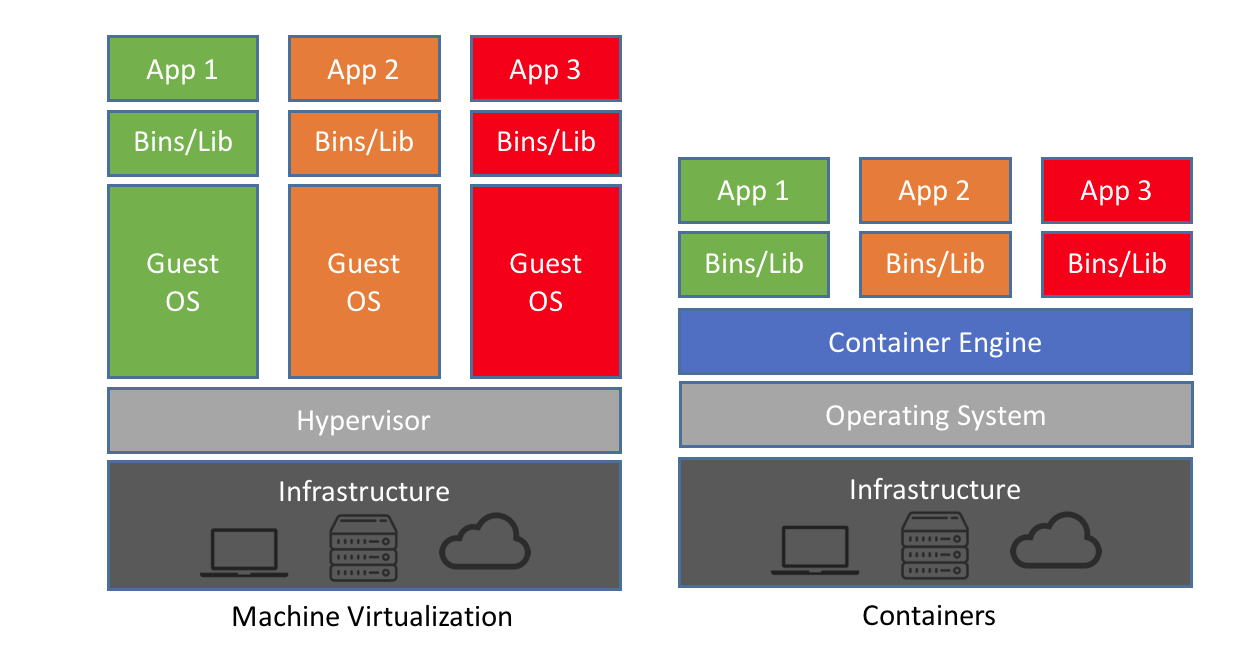
\includegraphics[width=0.55\textwidth]{images/cvm.png}
\end{center}

So the goal of your build process should be to produce a container that is ready to be deployed and managed by the other parts of your infrastructure (e.g., Kubernetes). 

Containers do potentially come with a downside of letting you just not upgrade things. Whereas before if you installed the OS patches you might get updates in your shared libraries, the container allows you to keep an old insecure version of a library around forever. So, don't do that. Keeping on top of security updates is important. Let's talk about that, actually, in the next course topic.

\bibliographystyle{alphaurl}
\bibliography{459}


\end{document}
